\documentclass[10pt,a4paper]{article}
\usepackage[utf8]{inputenc}
\usepackage[T1]{fontenc}
\usepackage[ngerman]{babel}
\usepackage{amsmath}
\usepackage{amsfonts}
\usepackage{amssymb}
\usepackage{graphicx}


\author{Gruppe 02}
\title{Pflichtenheft}
\begin{document}

	\subsection{Vorschlage}
	\subsection{Website}
	\begin{figure}[h]
		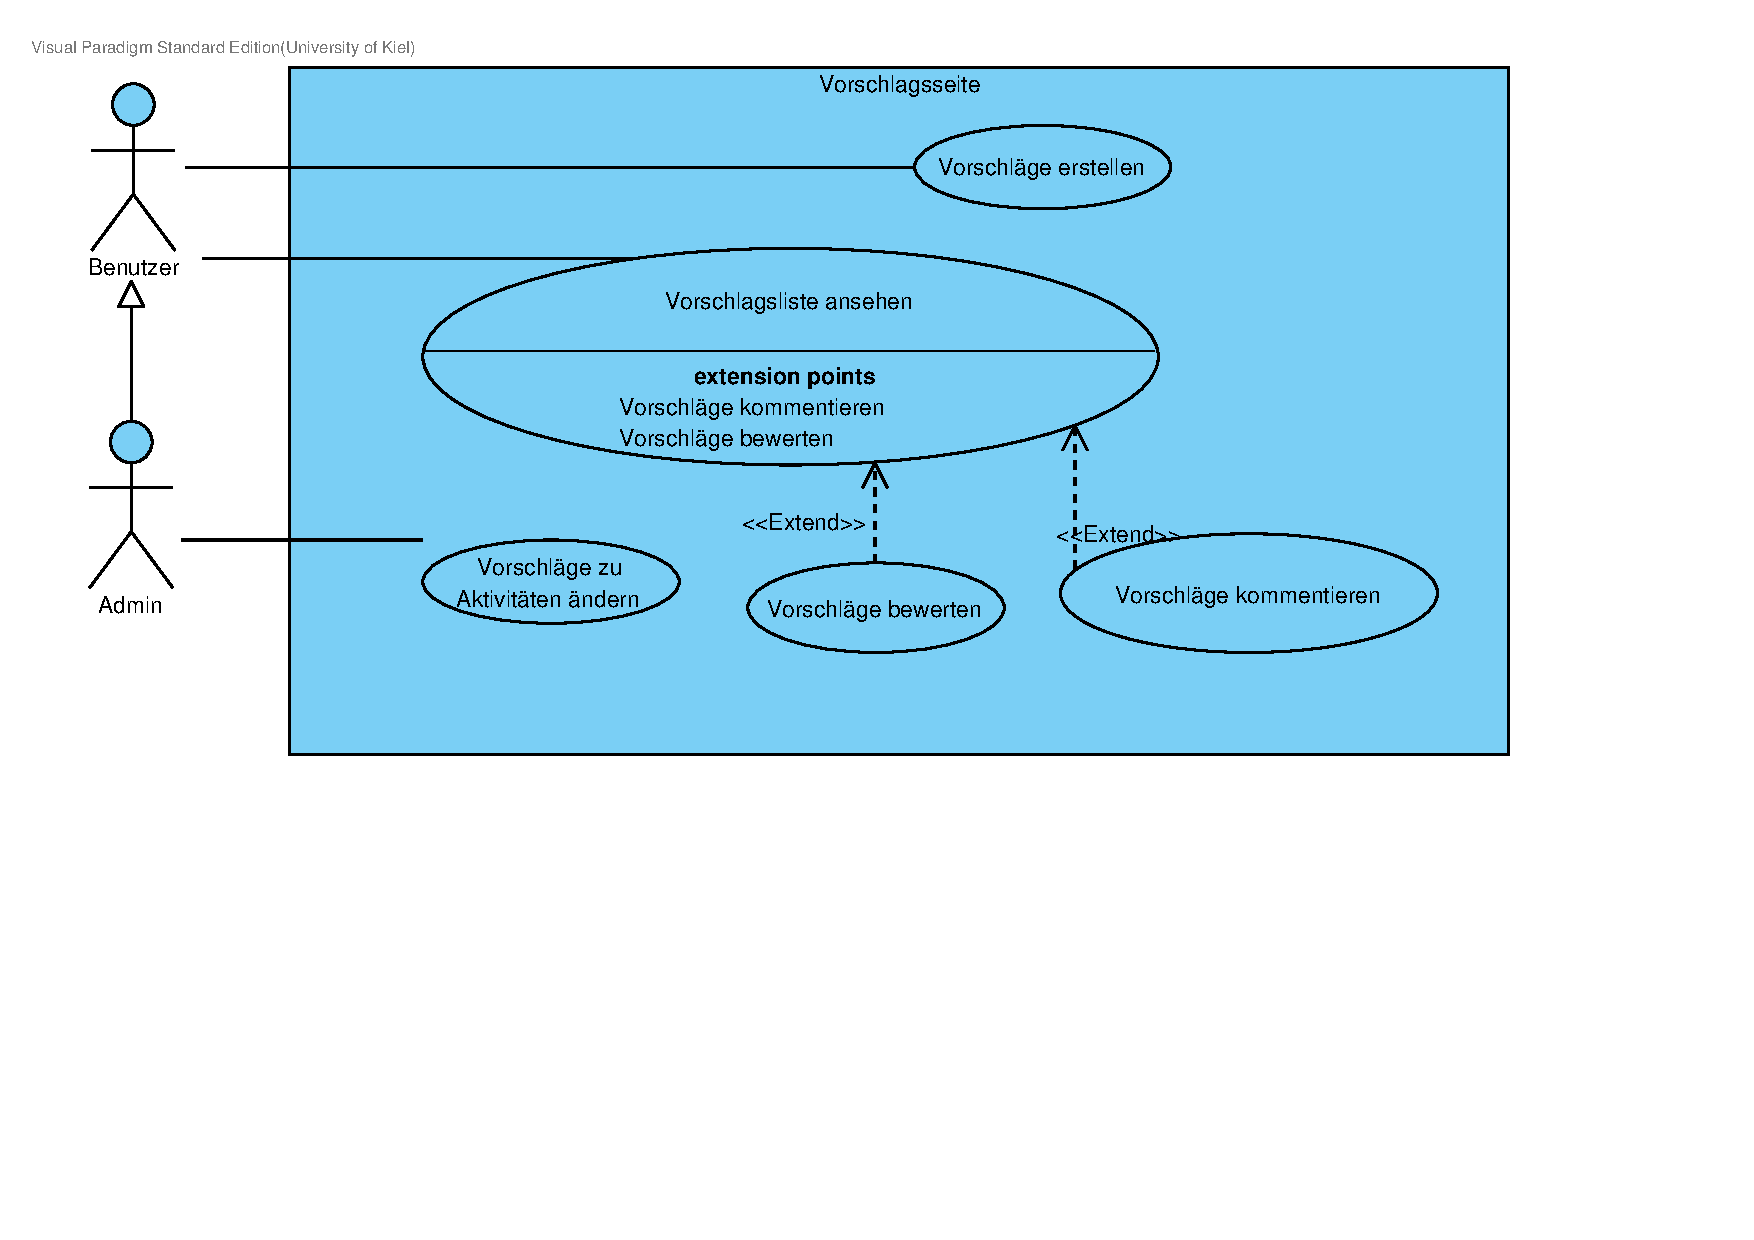
\includegraphics[width=\linewidth]{gfx/webseite/vorschlage.pdf}
	\end{figure}
	\subsubsection{Schaffen Vorschlage}
	\begin{tabular}{|l|p{.5\linewidth}|}
	\hline Use Case Nummer & - \\ 
	\hline Use Case Name & Schaffen Vorschlage \\ 
	\hline Initiierender Akteur & User \\
	\hline Weitere Akteure & \\
	\hline Kurzbeschreibung & The User fills out a form to create a proposal for a possible new activity. \\
	\hline Vorbedingung & Logged in as User \\
	\hline Nachbedingung & The user is then shown the page for their new proposal. \\
	\hline \multicolumn{2}{|c|}{Funktionalität des UseCases}\\
	\hline Ablauf & \begin{itemize}
			\item The user enters their proposal into a form (Title, Short Description, Points Value, Start Date and End Date)
			\item The User then submits their proposal which is then viewable.
		\end{itemize} \\ \\
	\hline Alternativen &  \\
	\hline Ausnahmen & \begin{itemize}
			\item If any of the required information is not entered the proposal is rejected.
			\item If the points value is not a valid integer the proposal is rejected.
			\item If either or both of the dates are invalid the proposal is rejected
		\end{itemize} \\
	\hline Benutzte Use Cases &  \\
	\hline \multicolumn{2}{|c|}{Weitere Informationen} \\
	\hline Spezielle Anforderungen &  \\
	\hline Annahmen &  \\
	\hline
	\end{tabular}
	
	\subsubsection{Sternen Wertung Vorschlage}
	\begin{tabular}{|l|p{.5\linewidth}|}
	\hline Use Case Nummer & - \\ 
	\hline Use Case Name & Sternen Wertung Vorschlage \\ 
	\hline Initiierender Akteur & User \\
	\hline Weitere Akteure & \\
	\hline Kurzbeschreibung & The User rates a submitted proposal on a scale of stars. \\
	\hline Vorbedingung & Logged in as User \\
	\hline Nachbedingung & The star rating is no longer clickable (to prevent multiple ratings by one user). \\
	\hline \multicolumn{2}{|c|}{Funktionalität des UseCases}\\
	\hline Ablauf & \begin{itemize}
			\item The user selects their star rating and clicks to submit the rating.
			\item the average rating given by users so far is then shown to the user.
		\end{itemize} \\ \\
	\hline Alternativen &  \\
	\hline Ausnahmen &  \\
	\hline Benutzte Use Cases & \begin{itemize}
			\item Liste Vorschlage
			\item Auswahlen Vorschlage
		\end{itemize} \\
	\hline \multicolumn{2}{|c|}{Weitere Informationen} \\
	\hline Spezielle Anforderungen &  \\
	\hline Annahmen &  \\
	\hline
	\end{tabular}
	
	\subsubsection{Kommentiert Vorschlage}
	\begin{tabular}{|l|p{.5\linewidth}|}
	\hline Use Case Nummer & - \\ 
	\hline Use Case Name & Kommentiert Vorschlage \\ 
	\hline Initiierender Akteur & User \\
	\hline Weitere Akteure & \\
	\hline Kurzbeschreibung & The User enters and submits a comment which is then viewable alongside a proposal. \\
	\hline Vorbedingung & Logged in as User \\
	\hline Nachbedingung & The comment area is longer usable (to prevent multiple unessicarry or unintended comments). \\
	\hline \multicolumn{2}{|c|}{Funktionalität des UseCases}\\
	\hline Ablauf & \begin{itemize}
			\item The user types out a comment.
			\item The user submits the comment.
			\item The comment is then shown in the appropriate section of the page.
		\end{itemize} \\ \\
	\hline Alternativen &  \\
	\hline Ausnahmen & \begin{itemize}
			\item If no text is entered the comment will be rejected.
			\item If the comment is too long it will be rejected.
		\end{itemize} \\
	\hline Benutzte Use Cases & \begin{itemize}
			\item Liste Vorschlage
			\item Auswahlen Vorschlage
		\end{itemize} \\
	\hline \multicolumn{2}{|c|}{Weitere Informationen} \\
	\hline Spezielle Anforderungen &  \\
	\hline Annahmen &  \\
	\hline
	\end{tabular}
	
	\subsubsection{Andern Vorschlage zu Aktivitaten}
	\begin{tabular}{|l|p{.5\linewidth}|}
	\hline Use Case Nummer & - \\ 
	\hline Use Case Name & Andern Vorschlage zu Aktivitaten \\ 
	\hline Initiierender Akteur & Admin \\
	\hline Weitere Akteure & \\
	\hline Kurzbeschreibung & The Admin selects a proposal. The Admin then confirms the change from a user proposal to an activity. \\
	\hline Vorbedingung & Logged in as Admin \\
	\hline Nachbedingung & \\
	\hline \multicolumn{2}{|c|}{Funktionalität des UseCases}\\
	\hline Ablauf & \begin{itemize}
			\item The Admin selects a proposal from a list of all proposals
			\item The Admin is then shown the proposal in full before confirming the change into an activity.
		\end{itemize} \\ \\
	\hline Alternativen &  \\
	\hline Ausnahmen & \\
	\hline Benutzte Use Cases & \begin{itemize}
			\item Liste Vorschlage
			\item Vorschlage Auswahlen
		\end{itemize} \\
	\hline \multicolumn{2}{|c|}{Weitere Informationen} \\
	\hline Spezielle Anforderungen &  \\
	\hline Annahmen &  \\
	\hline
	\end{tabular}
	
	\subsection{Android App}
	\begin{figure}[h]
		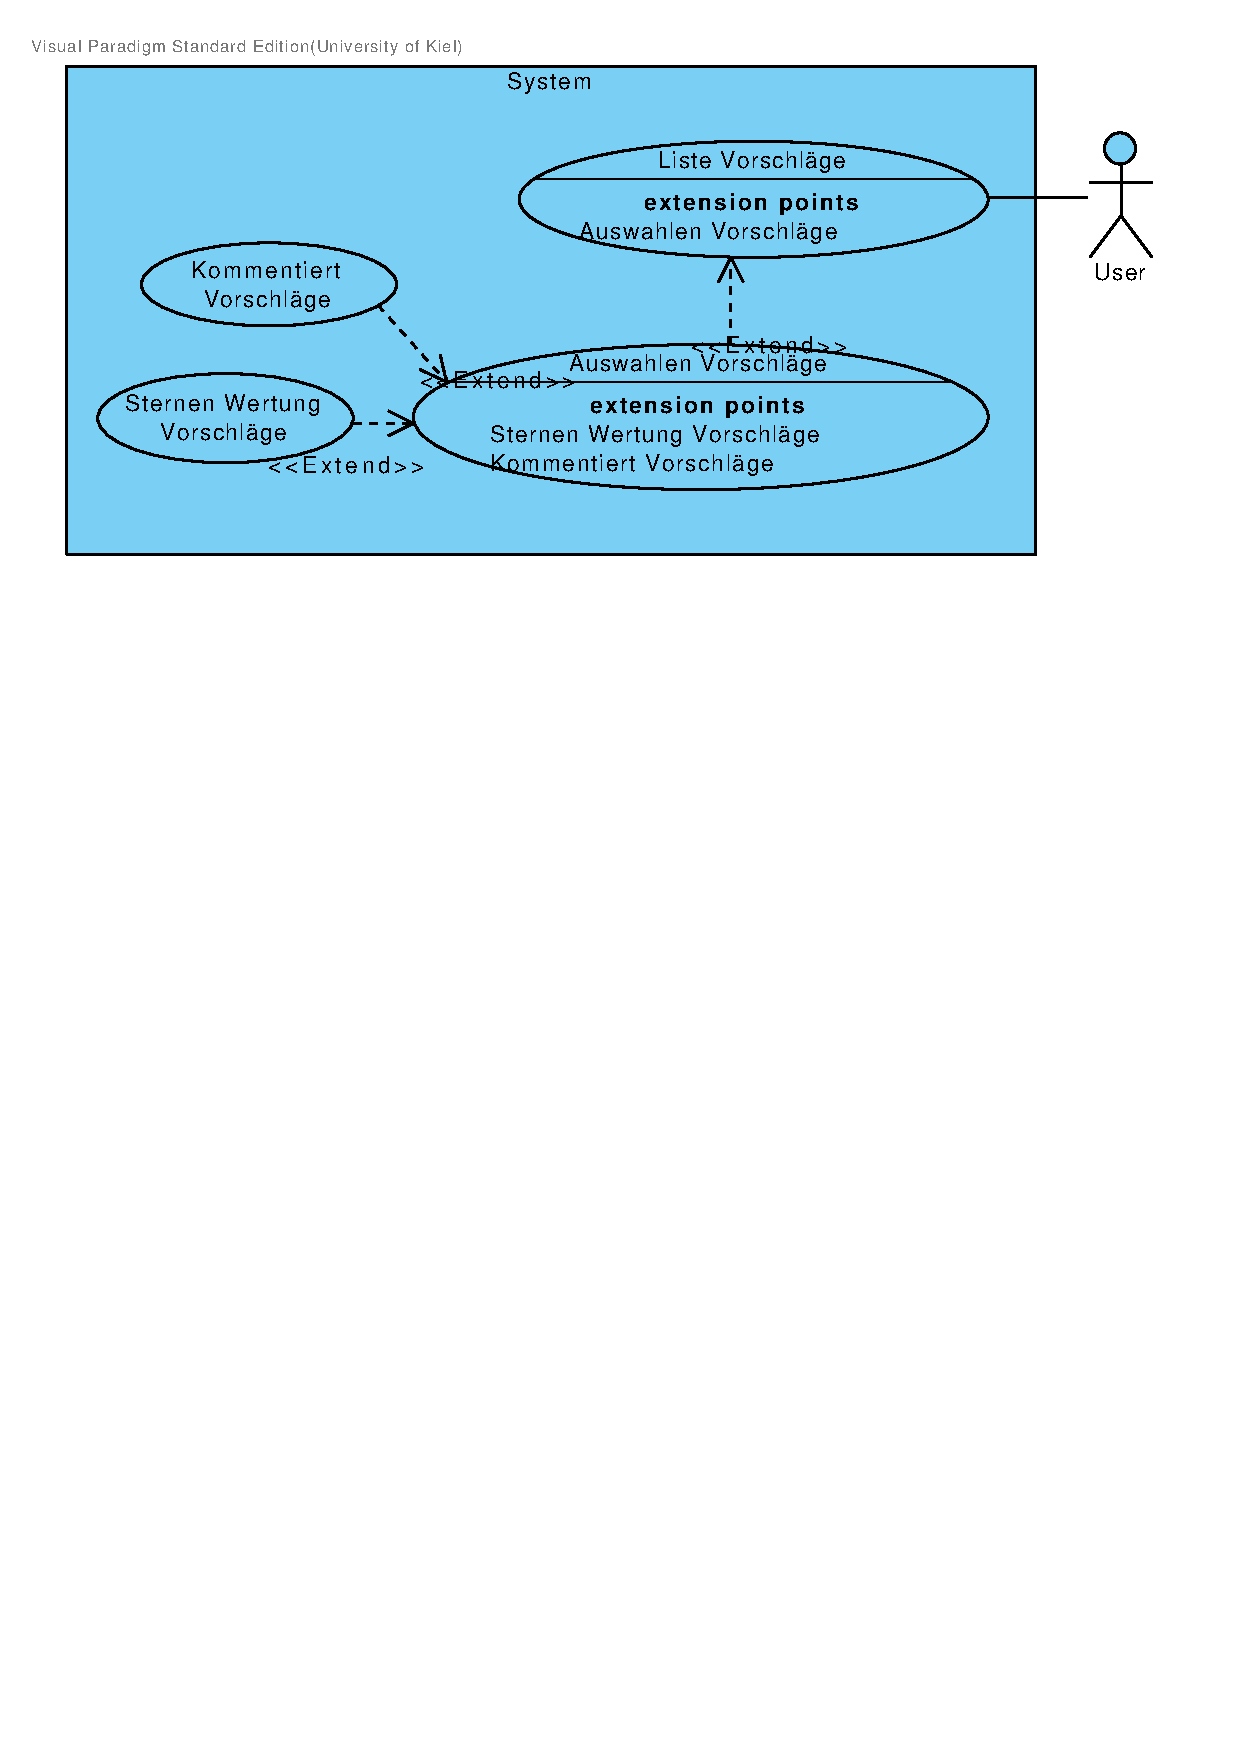
\includegraphics[width=\linewidth]{gfx/androidapp/vorschlage.pdf}
	\end{figure}
	\subsubsection{Schaffen Vorschlage}
	\begin{tabular}{|l|p{.5\linewidth}|}
	\hline Use Case Nummer & - \\ 
	\hline Use Case Name & Schaffen Vorschlage \\ 
	\hline Initiierender Akteur & User \\
	\hline Weitere Akteure & \\
	\hline Kurzbeschreibung & The User fills out a form to create a proposal for a possible new activity. \\
	\hline Vorbedingung & Logged in as User \\
	\hline Nachbedingung &  \\
	\hline \multicolumn{2}{|c|}{Funktionalität des UseCases}\\
	\hline Ablauf & \begin{itemize}
			\item The user enters their proposal into a form (Title, Short Description, Points Value, Start Date and End Date)
			\item The User then submits their proposal which is then viewable.
		\end{itemize} \\ \\
	\hline Alternativen &  \\
	\hline Ausnahmen & \begin{itemize}
			\item If any of the required information is not entered the proposal is rejected.
			\item If the points value is not a valid integer the proposal is rejected.
			\item If either or both of the dates are invalid the proposal is rejected
		\end{itemize} \\
	\hline Benutzte Use Cases &  \\
	\hline \multicolumn{2}{|c|}{Weitere Informationen} \\
	\hline Spezielle Anforderungen &  \\
	\hline Annahmen &  \\
	\hline
	\end{tabular}
	
	\subsubsection{Sternen Wertung Vorschlage}
	\begin{tabular}{|l|p{.5\linewidth}|}
	\hline Use Case Nummer & - \\ 
	\hline Use Case Name & Sternen Wertung Vorschlage \\ 
	\hline Initiierender Akteur & User \\
	\hline Weitere Akteure & \\
	\hline Kurzbeschreibung & The User rates a submitted proposal on a scale of stars. \\
	\hline Vorbedingung & Logged in as User \\
	\hline Nachbedingung & The rating scale is no longer usable (to prevent multiple ratings). \\
	\hline \multicolumn{2}{|c|}{Funktionalität des UseCases}\\
	\hline Ablauf & \begin{itemize}
			\item The user selects their rating along a scale of stars.
			\item The average rating given so far is then shown to the user.
		\end{itemize} \\ \\
	\hline Alternativen &  \\
	\hline Ausnahmen &  \\
	\hline Benutzte Use Cases & \begin{itemize}
			\item Liste Vorschlage
			\item Auswahlen Vorschlage
		\end{itemize} \\
	\hline \multicolumn{2}{|c|}{Weitere Informationen} \\
	\hline Spezielle Anforderungen &  \\
	\hline Annahmen &  \\
	\hline
	\end{tabular}
	
	\subsubsection{Kommentiert Vorschlage}
	\begin{tabular}{|l|p{.5\linewidth}|}
	\hline Use Case Nummer & - \\ 
	\hline Use Case Name & Kommentiert Vorschlage \\ 
	\hline Initiierender Akteur & User \\
	\hline Weitere Akteure & \\
	\hline Kurzbeschreibung & The User enters and submits a comment which is then viewable alongside a proposal. \\
	\hline Vorbedingung & Logged in as User \\
	\hline Nachbedingung & The comment box is no longer usable (to prevent multiple unessicarry or unintentional comments) \\
	\hline \multicolumn{2}{|c|}{Funktionalität des UseCases}\\
	\hline Ablauf & \begin{itemize}
			\item The user types out a comment.
			\item The user submits the comment.
			\item The new comment is then shown on the appropriate part of the screen.
		\end{itemize} \\ \\
	\hline Alternativen &  \\
	\hline Ausnahmen & \begin{itemize}
			\item If no text is entered the comment will be rejected.
			\item If the comment is too long it will be rejected.
		\end{itemize} \\
	\hline Benutzte Use Cases & \begin{itemize}
			\item Liste Vorschlage
			\item Auswahlen Vorschlage
		\end{itemize} \\
	\hline \multicolumn{2}{|c|}{Weitere Informationen} \\
	\hline Spezielle Anforderungen &  \\
	\hline Annahmen &  \\
	\hline
	\end{tabular}

\end{document}